% Chapter Template

% Main chapter title
%\chapter[toc version]{doc version}
\chapter{Background}

% Short version of the title for the header
%\chaptermark{version for header}

% Chapter Label
% For referencing this chapter elsewhere, use \ref{ChapterTemplate}
\label{Section2}\label{chap:background}

% Write text in here
% Use \subsection and \subsubsection to organize text
This chapter introduces the theoretical background necessary to understand the contributions of this work. 
We first provide an overview of the Transformer architecture, which underpins most modern LLMs~\cite{minaee2024large}. 
We then discuss the challenge of representing natural language text as input for these models, tracing the evolution of tokenization algorithms and their role in large-scale language modeling.


\section{Transformers}\label{Section2.2}

The task of enabling machines to process and understand natural language has long been a central challenge in artificial intelligence research \cite{harris1954distributional}.
Early approaches were primarily rule-based, relying on hand-crafted grammars and symbolic systems that proved brittle, unable to capture the variability and richness of human language \cite{winograd1972understanding}.
The introduction of statistical methods and later neural models marked a turning point, allowing researchers to capture patterns of co-occurrence and semantic regularities in a data-driven manner~\cite{bengio2003neural}.

A key milestone was the development of distributed word representations, motivated by the distributional hypothesis that words appearing in similar contexts tend to have similar meanings \cite{harris1954distributional}. Instead of treating words as discrete symbols, models such as \texttt{word2vec} \cite{mikolov2013efficient} and \texttt{GloVe} \cite{pennington2014glove} learned dense vector embeddings that captured semantic similarity. These representations proved powerful in downstream tasks such as text classification \cite{zhang2015character}, sentiment analysis \cite{socher2013recursive}, and machine translation \cite{zhang2015character}.
However, these embeddings were \textit{static} -- i.e., the word “bank” had the same representation whether it referred to a riverbank or a financial institution -- making them insufficient for capturing context-dependent meaning \cite{dai2019transformerxlattentivelanguagemodels}.


The search for context-sensitive representations led to the rise of deep neural architectures for sequence modeling. Recurrent Neural Networks (RNNs) \cite{elman1990finding} and their variants, such as LSTMs \cite{hochreiter1997long} and GRUs \cite{chung2014empirical}, introduced hidden states that evolved with the sequence, allowing models to adapt word representations based on preceding tokens. This enabled breakthroughs in tasks such as language modeling and machine translation \cite{sutskever2014sequence}. Yet these models had inherent limitations: they struggled with long contexts due to vanishing gradients, relied on sequential computation that restricted parallelization, and became increasingly inefficient as model sizes grew \cite{bengio1994learning,pascanu2013construct}.

Convolutional architectures offered an alternative \cite{kalchbrenner2014convolutional, gehring2017convolutional}, but they were primarily effective at modeling local patterns in text rather than capturing global semantic relationships \cite{johnson2017deep}. By the late 2010s, the core challenges in NLP still remained \cite{goldberg2018neural}: neural networks struggled to balance scalability with robust handling of linguistic ambiguity and discrete symbolic structure.

However, these challenges were mitigated with the introduction of the Transformer architecture by \citet{vaswani2017attention}. The Transformer replaced recurrence and convolutions with a novel mechanism: \textit{self-attention}. Instead of processing text sequentially, self-attention allowed the model to directly relate each token to every other token in the sequence, regardless of distance. This architecture addressed several bottlenecks simultaneously: it scaled efficiently by enabling parallel training across entire sequences \cite{vaswani2017attention}, captured long-range dependencies more effectively than RNNs or CNNs \cite{tang2019distilling}, and produced contextualized word embeddings, where the representation of a word adapts dynamically to its contextual environment \cite{peters-etal-2018-deep}. Together, these innovations reshaped the possibilities in NLP~\cite{wolf2020transformers}.

Despite its adoption not being instantaneous, it gained momentum as subsequent models demonstrated their capabilities at scale. Within just a few years, the architecture became the backbone of nearly all modern large-scale language models \cite{wolf2020transformers}.The original Transformer paper has since been cited over 190,000 times (as of September 2025), and the architecture underpins influential models such as BERT \cite{devlin2019bert}, the GPT series \cite{radford2018improving, brown2020language}, T5 \cite{raffel2020exploring}, and more recent open-source efforts such as LLaMA \cite{touvron2023llama} and Mistral \cite{jiang2023mistral7b}. These systems collectively demonstrated that scaling Transformer architectures could yield unprecedented performance across virtually every NLP benchmark.


\begin{figure}[H]
    \centering
    \scalebox{0.8}{ % scale down to 80%
        \begin{tikzpicture}[
            timeline/.style={thick, draw=black, -latex},
            event/.style={
                rectangle,
                rounded corners,
                draw=black,
                fill=gray!10,
                align=center,
                text width=2.8cm,
                font=\scriptsize
            }
        ]
        
            % Timeline line
            \draw[timeline] (0,0) -- (15,0);
            
            % Events
            \node[event, above=0.4cm of {(0,0)}] {1950s–70s\\Rule-based NLP\\\cite{winograd1972understanding}};
            \node[event, below=0.4cm of {(3,0)}] {1990s\\Statistical NLP + RNNs\\\cite{elman1990finding}};
            \node[event, above=0.4cm of {(6,0)}] {2013–14\\Word2Vec, GloVe\\\cite{mikolov2013efficient,pennington2014glove}};
            \node[event, below=0.4cm of {(8.5,0)}] {2014–15\\Seq2Seq, CNNs\\\cite{sutskever2014sequence,kim2014convolutional}};
            \node[event, above=0.4cm of {(11,0)}] {2017\\Transformer\\\cite{vaswani2017attention}};
            \node[event, below=0.4cm of {(13,0)}] {2018–20\\BERT, GPT, T5\\\cite{devlin2019bert,radford2018improving,raffel2020exploring}};
            \node[event, above=0.4cm of {(15,0)}] {2023+\\LLaMA, Mistral, GPT-4\\\cite{touvron2023llama,jiang2023mistral7b}};
            
        \end{tikzpicture}
    } % end scale
    \caption{Timeline of major milestones in NLP leading to Transformer-based LLMs.}
    \label{fig:nlp-timeline}
\end{figure}


% % VERTICAL TIMELINE
% \begin{figure}[H]
%     \centering
%     \begin{tikzpicture}[
%         timeline/.style={thick, draw=black},
%         event/.style={
%             rectangle,
%             rounded corners,
%             draw=black,
%             fill=gray!10,
%             align=center,
%             text width=5cm,
%             font=\small
%         }
%     ]
    
%         % Timeline line
%         \draw[timeline] (0,0) -- (0,-14);
        
%         % Events
%         \node[event, right=0.5cm of { (0,0) }] {1950s–70s\\Rule-based NLP\\\cite{winograd1972understanding}};
%         \node[event, left=0.5cm of { (0,-2.5) }] {1990s\\Statistical NLP + RNNs\\\cite{elman1990finding}};
%         \node[event, right=0.5cm of { (0,-5) }] {2013–14\\Word2Vec, GloVe\\\cite{mikolov2013efficient,pennington2014glove}};
%         \node[event, left=0.5cm of { (0,-7.5) }] {2014–15\\Seq2Seq, CNNs for NLP\\\cite{sutskever2014sequence,kim2014convolutional}};
%         \node[event, right=0.5cm of { (0,-10) }] {2017\\Transformer\\\cite{vaswani2017attention}};
%         \node[event, left=0.5cm of { (0,-12.5) }] {2018–20\\BERT, GPT, T5\\\cite{devlin2019bert,radford2018improving,raffel2020exploring}};
%         \node[event, right=0.5cm of { (0,-15) }] {2023+\\LLaMA, Mistral, GPT-4\\\cite{touvron2023llama,jiang2023mistral7b}};
    
%     \end{tikzpicture}
%     \caption{Timeline of major milestones in natural language processing leading to Transformer-based LLMs.}
%     \label{fig:nlp-timeline-vertical}
% \end{figure}



% \begin{figure}[H]
%     \centering
%       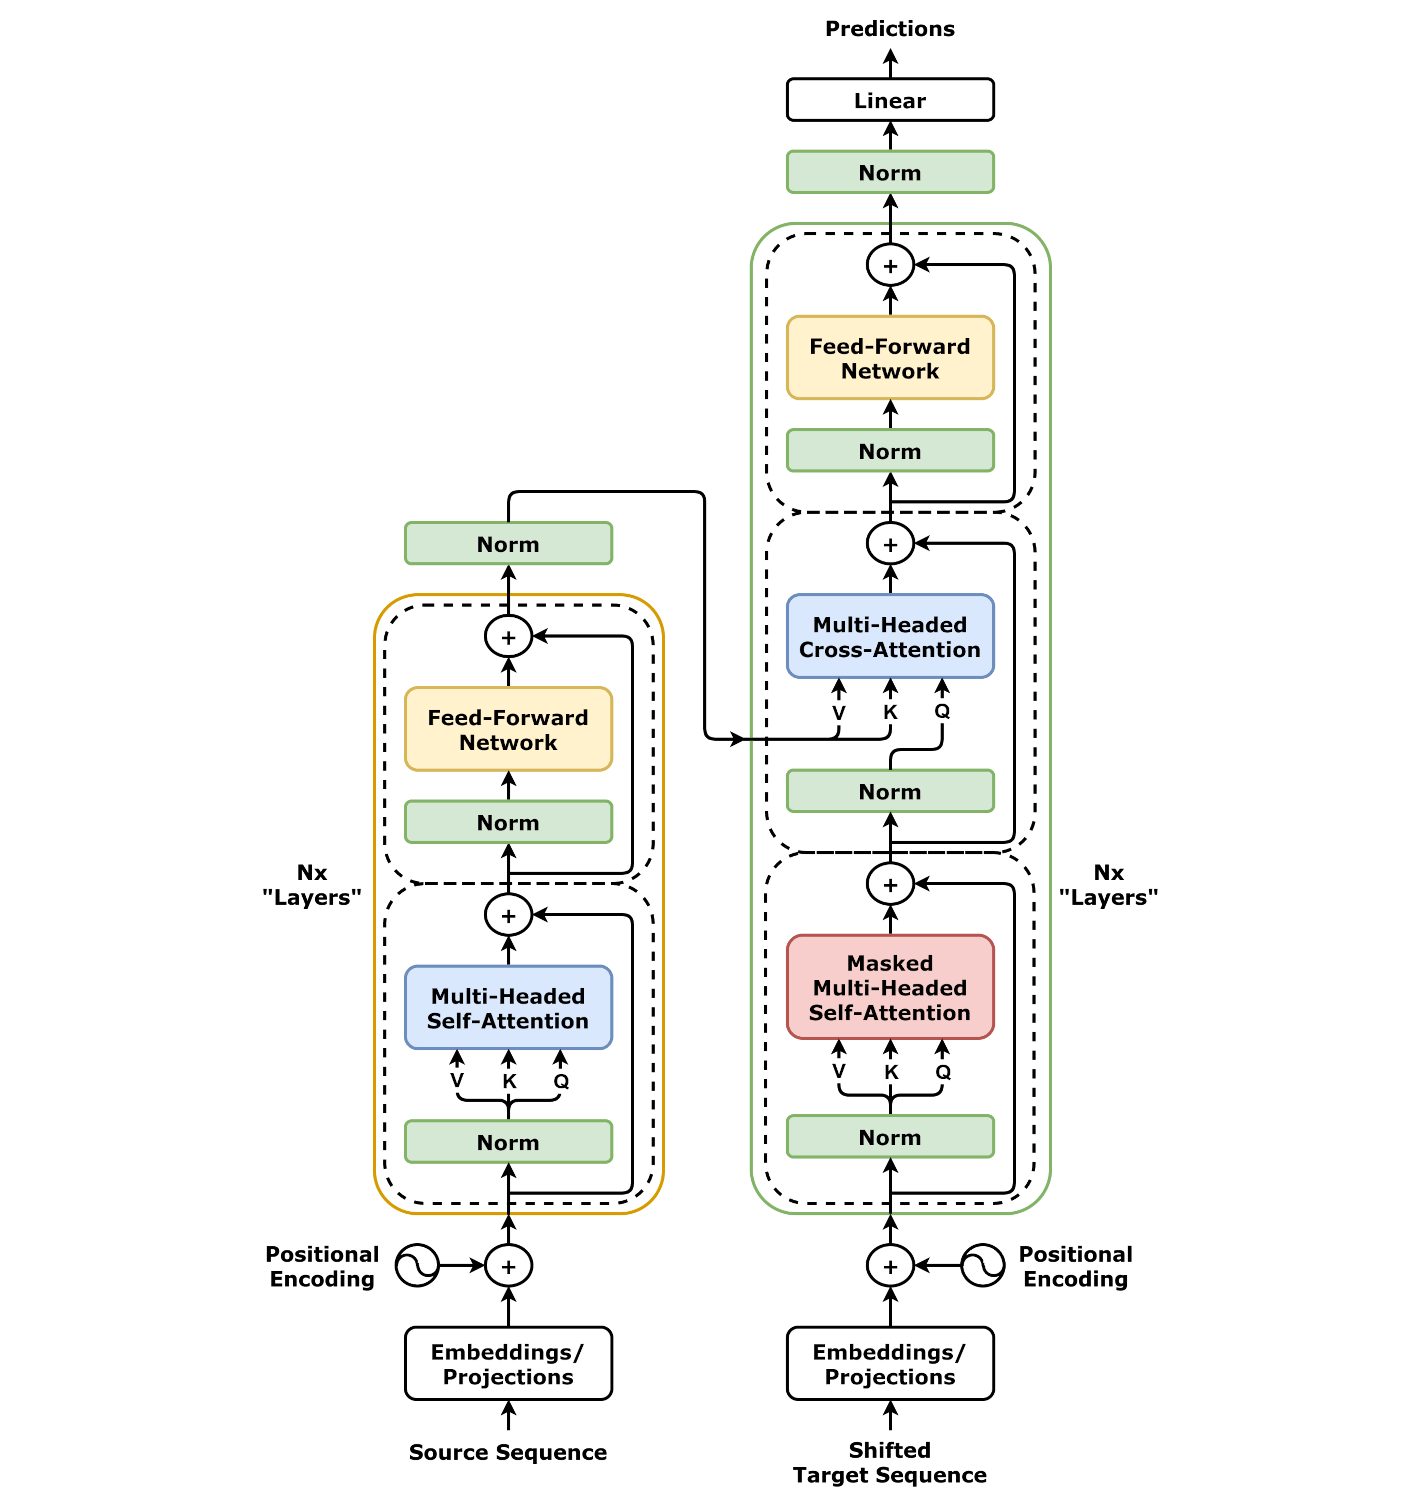
\includegraphics[width=0.5\columnwidth]{Transformers/full_architecture.png}
%       \captionof{figure}{\label{fig:Transformers-FullArchitecture}Transformer architecture - \href{https://en.wikipedia.org/wiki/Transformer_(deep_learning_architecture)}{https://en.wikipedia.org/wiki/Transformer\_(deep\_learning\_architecture)}}
% \end{figure}

A Transformer model processes data through several conceptual stages. The input data first goes through multiple layers in the \textbf{encoder stack}. The first layer that the data goes through is the \emph{Embedding Layer}, followed by multiple stacked layers of self-attention and feedforward networks, producing context-sensitive representations of the sequence. Finally, task-specific output layers allow the model to generate text, classify sequences, or perform other downstream tasks. 

As this dissertation is primarily concerned with adapting the \emph{Tokenizer} and \emph{Embedding} layers for cross-lingual use, we provide a more detailed discussion of these components in the following sections.



\subsection{Embedding}\label{Section2.2.4}
The Transformer requires inputs in the form of numerical vectors of a fixed dimension. Prior to entering the model, inputs are mapped into this vector space through an \emph{Embedding Layer} or equivalent projection step.

Each input element is passed through an embedding matrix -- a learnable parameter of the model -- which maps it to a dense vector of fixed size. These vectors are referred to as \textit{embeddings}.

% Let \( V \) be the vocabulary size and \( d \) be the embedding dimension. The embedding layer is a matrix \( E \in \mathbb{R}^{V \times d} \), where each row corresponds to the embedding of a token. For an input sequence of token IDs \( [t_1, t_2, \dots, t_n] \), the embedding layer outputs:

% \[
% \mathbf{X} = [E_{t_1}; E_{t_2}; \dots; E_{t_n}] \in \mathbb{R}^{n \times d}
% \]

They are then augmented with \textbf{positional encodings} to provide information about the order of elements in the sequence, as the transformer architecture has no inherent notion of order.

% \paragraph{Role in Transformer Models} The embedding layer is the entry point of the transformer model. This layer allows the translation of input sequences onto high-dimensional vector spaces which allows the model to retain information on input sequences. Pre-trained Transformer models, such as BERT~\cite{devlin2019bert} and GPT-2~\cite{radford2019language}, use embeddings trained on large corpora, which encode rich semantic and syntactic information.

\paragraph{Modifying the Embedding Layer.} In this dissertation, only the \emph{Embedding Layer} is trained during the adaptation of a large language model to a new language. This is a form of lightweight fine-tuning, where the embedding matrix is modified while keeping the rest of the model frozen. This strategy is computationally efficient and has demonstrated effectiveness in low-resource or domain adaptation settings~\cite{artetxe2019cross}.

By adjusting only the \emph{Embedding Layer}, we aim to \textit{re-align} the model's input space without requiring full model retraining.


\subsection{Attention Layer}\label{Section2.2.3}\label{subsec:attention-layer}
During the attention layer, the model learns dependencies between input elements by computing how much each element should attend to every other element in the sequence. 

Concretely, the inputs (represented as embeddings) are projected into three sets of vectors: queries, keys, and values. Attention weights are obtained by computing the dot product of queries and keys, scaling the result, and applying a softmax function to normalize the weights. These weights are then used to compute a weighted sum of the values, producing context-aware representations for each input element.

This mechanism allows the model to dynamically incorporate information from the entire input sequence at every layer, enabling it to capture complex relationships across long-context windows.


\subsection{Decoding}\label{Section2.2.2}
Once the input elements have been converted into embeddings and processed through the self-attention and feedforward layers, the decoder generates output representations that capture contextual relationships within the input sequence.  

The decoder typically consists of multiple layers, each containing a self-attention mechanism and a feedforward network. These layers iteratively refine the input representations, allowing the model to capture complex dependencies across the entire sequence.

Finally, the decoder produces a probability distribution over the model's output space (e.g., vocabulary in language tasks), which can then be used to select or generate the next element in the output sequence. This process is repeated auto-regressively for sequence generation tasks or directly applied to classification or regression.


\section{Tokenizers}\label{Section2.1}

% -----------------------------
% The Problem of Text Encoding
% -----------------------------
While the Transformer architecture itself operates on continuous vectors, natural language consists of discrete symbolic units (characters). 
Thus, to apply Transformers to text, one must first answer the question: \emph{How can we represent text in a form suitable for Transformer models?} This question raises the problem of designing a procedure to convert raw strings into sequences of numerical identifiers.

Early solutions to this problem arose not from NLP, but from data compression research. Algorithms such as Byte Pair Encoding (BPE) \cite{gage1994new} were originally introduced as general-purpose compression methods, designed to replace frequent symbol pairs with a more space-effective value (e.g., a single 8-bit number) but were later adapted to construct vocabularies of variable-length subword units, balancing vocabulary size and coverage.

By utilizing algorithms such as BPE, it becomes possible to map character strings into sequences of discrete tokens, which are then mapped into vectors through the \emph{Embedding Layer}. The list of tokens present in a tokenizer defines the ``vocabulary'' of the model and serves as the entry point for any language processing task.


Formally:
$$
T : \Sigma^* \rightarrow V^k, \quad S \mapsto (t_1, t_2, \dots, t_k)
$$
where $\Sigma$ is the alphabet (e.g., Unicode characters), $\Sigma^*$ is the set of all finite strings over $\Sigma$, and $V \subset \Sigma^*$ is the vocabulary.

\subsection{Tokenization Process}
The general tokenization pipeline consists of the following stages:

\begin{algorithm}[H]
\caption{Generic Tokenization Process}
\begin{algorithmic}[1]
\State \textbf{Input:} Text string $S$
\State Preprocessing (optional): lowercase, Unicode normalization, whitespace handling
\State Splitting: divide text into basic units (e.g., \texttt{"cat"} → [\texttt{cat}]; \texttt{"cat"} → [\texttt{c}, \texttt{at}]; \texttt{"cat"} → [\texttt{c}, \texttt{a}, \texttt{t}])
\State Mapping: assign token IDs via vocabulary lookup
\State Add special tokens: [CLS], [SEP], [PAD], etc. (if required by the model)
\State \textbf{Output:} Token sequence $(t_1, t_2, \dots, t_n)$
\end{algorithmic}
\end{algorithm}


Subword tokenization has been the predominant choice for most recent LLMs since it balances vocabulary size and handling of out-of-vocabulary words~\cite{sennrich2015neural, wu2016google, kudo2018sentencepiece, bostrom2020byte}.

% -----------------------------
% Byte-Pair Encoding (BPE)
% -----------------------------
\subsection{Byte-Pair-Encoding (BPE)}\label{Section2.1.2}\label{subsec:byte-pair-encoding_bpe}
    The BPE algorithm’s original purpose -- storage optimization -- was achieved by iteratively replacing the most frequent pairs of bytes in a sequence with a new symbol of smaller size. This simple frequency-based merging strategy was later adapted to natural language processing by \citet{sennrich2015neural}, where the goal was no longer to compress text, but to efficiently build a vocabulary of subword units for machine translation systems.
    
    The key motivation for BPE in NLP is its balance between two extremes: word-level vocabularies, which suffer from out-of-vocabulary (OOV) issues, and character-level vocabularies, which lead to excessively long sequences. By iteratively merging frequent character pairs into larger units, BPE naturally captures common morphemes, prefixes, and suffixes (e.g., merging ``ing'' or ``pre'' as reusable subword units). This property makes it well-suited for handling rare words, inflected forms, and domain-specific terminology.
    
    \paragraph{Illustrative Example.}
    Consider the word “lower”. With a character-level vocabulary, it is split as [\texttt{l}, \texttt{o}, \texttt{w}, \texttt{e}, \texttt{r}]. After training with BPE, frequent merges such as [\texttt{lo}] and [\texttt{wer}] might appear in the vocabulary, allowing the word to be represented as [\texttt{lo}, \texttt{wer}]. This reduces sequence length while preserving reconstructability of the original string.
    
    \paragraph{Algorithm.}  
    The algorithm can be summarized as follows:

    \begin{algorithm}[H]
    \caption{Byte-Pair Encoding (BPE)}
    \begin{algorithmic}[1]
    \State \textbf{Input:} Corpus $C$, size of target vocabulary $size$
    \State $V \gets$ set of all characters in $C$
    \State $R \gets \emptyset$
    \While{$|V| < size$}
        \State $P \gets$ Frequency Pairs in $C$
        \State $(A, B) \gets$ most frequent pair in $P$
        \State $R \gets R \cup \{(A, B)\}$
        \State $C \gets replace(C, (A,B), Z)$, where $Z = concat(A, B)$
        \State $V \gets V \cup \{AB\}$
    \EndWhile
    \State \textbf{Return:} $R$, Merge rules (e.g., "e" + "s" $\rightarrow$ "es").
    \end{algorithmic}
    \end{algorithm}


% -----------------------------
% WordPiece
% -----------------------------
\subsection{WordPiece}\label{Section2.1.3}
    WordPiece was first introduced in the context of statistical machine translation \cite{schuster2012japanese} and later became widely adopted in large-scale pre-trained models such as BERT \cite{devlin2019bert}. Like BPE, it builds a subword vocabulary by iteratively merging symbols. However, instead of relying purely on frequency, WordPiece selects merges that maximize the likelihood of the training corpus under a language model. This makes it more sensitive to semantic and syntactic regularities than raw frequency counts.

    The intuition behind WordPiece is to prefer merges that result in subword units useful for predicting text. For instance, while BPE may merge frequent pairs regardless of context, WordPiece evaluates whether a candidate merge improves the probability of the corpus. This often leads to linguistically meaningful units being preserved, enhancing generalization to rare or unseen words.
    
    \paragraph{Illustrative Example.}
    Suppose the corpus contains words like \texttt{play}, \texttt{playing}, and \texttt{player}. WordPiece may merge \texttt{play} into a unit because doing so helps model all three words more compactly, while still leaving suffixes like \texttt{\#\#ing} or \texttt{\#\#er} as separate tokens.
    \paragraph{Algorithm.}  
    A simplified version of the procedure is shown below:
    
    \begin{algorithm}
    \caption{WordPiece}
    \begin{algorithmic}[1]
    \State \textbf{Input:} Corpus $C$, size of target vocabulary $size$
    \State $V \gets$ set of all characters in $C$
    \While{$|V| < size$}
        \State $scores = \{\}$
        \ForAll{candidate merges $(A,B)$ in $C$}
            \State $scores[(A,B)] \gets \frac{\text{freq}(AB)}{\text{freq}(A)\cdot \text{freq}(B)}$ \Comment{Likelihood-based scoring function}
        \EndFor
        \State $(A,B) \gets$ pair with highest score from $scores$
        \State $C \gets replace(C, (A,B), Z)$, where $Z = concat(A, B)$
        \State $V \gets V \cup \{AB\}$
    \EndWhile
    \State \textbf{Return:} $V$, Subword vocabulary
    \end{algorithmic}
    \end{algorithm}

    WordPiece remains the standard tokenization method in the Transformer family of models built for bidirectional pre-training, including BERT \cite{devlin2019bert}, DistilBERT \cite{sanh2019distilbert}, and ALBERT \cite{lan2019albert}, where efficient handling of rare words and morphological variations is critical.



% \paragraph{Advantages.}
% \begin{itemize}
%     \item \textbf{Efficiency:} Requires updating only a small fraction of model parameters.
%     \item \textbf{Modularity:} Allows swapping or re-learning embeddings without disturbing the rest of the model.
%     \item \textbf{Applicability:} Particularly useful when adapting to new tokenizers or vocabularies, as in this dissertation.
% \end{itemize}
